%%%%%%%%%%%%%%%%%%%%%%%%%%%%%%%%%%%%%%%%%%%%%%%%%%%%%%%%%
%%             东南大学电路实验报告 LaTeX 模板
%%                SEU-Circuit-Report.cls
%% https://github.com/Teddy-van-Jerry/SEU_Circuit_Report
%% ======================================================
%% 版本信息:
%% v1.1 (Oct. 24, 2021)
%% ------------------------------------------------------
%% 模板制作:
%% Teddy van Jerry, (me@teddy-van-jerry.org)
%% * GitHub: https://github.com/Teddy-van-Jerry
%% * Website: https://teddy-van-jerry.org
%% * Blog: https://blog.teddy-van-jerry.org
%% ------------------------------------------------------
%% 使用说明:
%% 1. 编译使用 XeLaTeX 和 Biber
%% 2. 报告基本信息通过修改导言区以 exp 开头的命令
%% 3. 参考文献位于 ref/ref.bib
%% 4. 报告模板依据 MIT License 开源共享
%% ------------------------------------------------------
%% Copyright 2021 (c) Teddy van Jerry
%%
%% Permission is hereby granted, free of charge, to any
%% person obtaining a copy of this software and
%% associated documentation files (the "Software"), to
%% deal in the Software without restriction, including
%% without limitation the rights to use, copy, modify,
%% merge, publish, distribute, sublicense, and/or sell
%% copies of the Software, and to permit persons to whom
%% the Software is furnished to do so, subject to the
%% following conditions:
%%
%% The above copyright notice and this permission notice
%% shall be included in all copies or substantial
%% portions of the Software.
%% 
%% THE SOFTWARE IS PROVIDED "AS IS", WITHOUT WARRANTY OF
%% ANY KIND, EXPRESS OR IMPLIED, INCLUDING BUT NOT
%% LIMITED TO THE WARRANTIES OF MERCHANTABILITY, FITNESS
%% FOR A PARTICULAR PURPOSE AND NONINFRINGEMENT. IN NO
%% EVENT SHALL THE AUTHORS OR COPYRIGHT HOLDERS BE LIABLE
%% FOR ANY CLAIM, DAMAGES OR OTHER LIABILITY, WHETHER IN
%% AN ACTION OF CONTRACT, TORT OR OTHERWISE, ARISING
%% FROM, OUT OF OR IN CONNECTION WITH THE SOFTWARE OR THE
%% USE OR OTHER DEALINGS IN THE SOFTWARE.
%%%%%%%%%%%%%%%%%%%%%%%%%%%%%%%%%%%%%%%%%%%%%%%%%%%%%%%%%%

%% 使用实验报告模板类(字体大小 12pt 最适合)
\documentclass[12pt]{SEU-Circuit-Report}

%%%%%%%%%%%%%%%%%%%% 报告基本信息 %%%%%%%%%%%%%%%%%%%%
\expno{3} % 实验序号
\expname{基于verilog的自动售货机} % 实验名称
\exphouse{吴健雄学院} % 学院
\expauthor{李勃璘(61522529)} % 姓名
\expmates{冯光宇(61522527)} % 同组人员
\expdate{2021年10月19日} % 实验日期
\expgrade{} % 成绩评定
\exptutor{翟建锋} % 评阅老师
%%%%%%%%%%%%%%%%%%%%%%%%%%%%%%%%%%%%%%%%%%%%%%%%%%%%

%% 定义附录命令
\renewcommand\appendix{\par
    \setcounter{section}{0}
    \setcounter{subsection}{0}
    \gdef\thesection{附录 \Alph{section}}}
%% 报告正文
\begin{document}
    % 打印封面页
    \exptitlepage
    \section{课题背景}
    自动售货机是一种无需人工服务的设备,消费者可以通过它自动购买各种商品。通常,自动售货机内部装有商品(如饮料、零食、日常用品等),通过投币、纸币、刷卡、移动支付等方式支付后,机器会自动将选择的商品提供给消费者。
    \section{FPGA与Vivado简介}
    
    \subsection{FPGA简介}
    现场可编程逻辑器件 (FPGA, Field Programmable Gate Array) 是一种集成电路可编程逻辑器件,它具有高灵活性、高可靠性、低功耗、高速度等特点,适合作为数字系统硬件设计的核心部件。利用FPGA,可以实现复杂的功能,如图像处理、视频处理、音频处理、机器人控制等,已经成为电子信息领域仿真、测试、验证的重要工具。

    本设计中,我们将采用NEXY4 4 DDR 型号的主板作为主控芯片。它基于Artix-7 FPGA系列,具有多种接口,如VGA、USB、Ethernet接口,同时允许16位拨片输入信号,5个按钮,以及两个复位键,支持用户自定义,能够满足自动售货机的设计需求。
    \subsection{Vivado简介}
    Vivado是一款基于Xilinx FPGA的集成开发环境,它是一款功能强大、界面简洁、操作方便的集成开发环境。本实验将使用\texttt{Vivado 2017.4} 版本进行设计,并作为仿真及测试软件进行自动售货机的设计。
    \section{自动售货机功能介绍}
    \subsection{功能概述}
    该项目的目标是设计一款基于FPGA的自动售货机,该自动售货机具有以下功能:
    \begin{enumerate}
        \item 商品选择:用户可以通过按下按钮选择商品,并将其放入“购物车”。允许用户每次最多选择两件商品(数量不限)。
        \item 结账:用户可以在购买的过程中随时结算“购物车”中的商品,此时系统进入结账环节。支持用户使用1元、5元、10元、20元、50元进行支付,并支持溢出找零。
        \item 找零:用户在结账过程中,若购物金额超过支付金额,系统将自动给用户找零。规定用户每次找零不超过1元,直至找零完毕。
        \item 退出:用户可以在任意时刻退出系统,系统将自动清空“购物车”中的商品并退回至空闲状态。
    \end{enumerate}
    \subsection{系统流程图}
    为了让自动售货机的工作流程更加清晰,便于用户理解该系统的工作原理,以及理清各个状态之间的关系,我们设计了下面的系统流程图,便于后续参考:
    \begin{figure}[htbp]
        \centering
        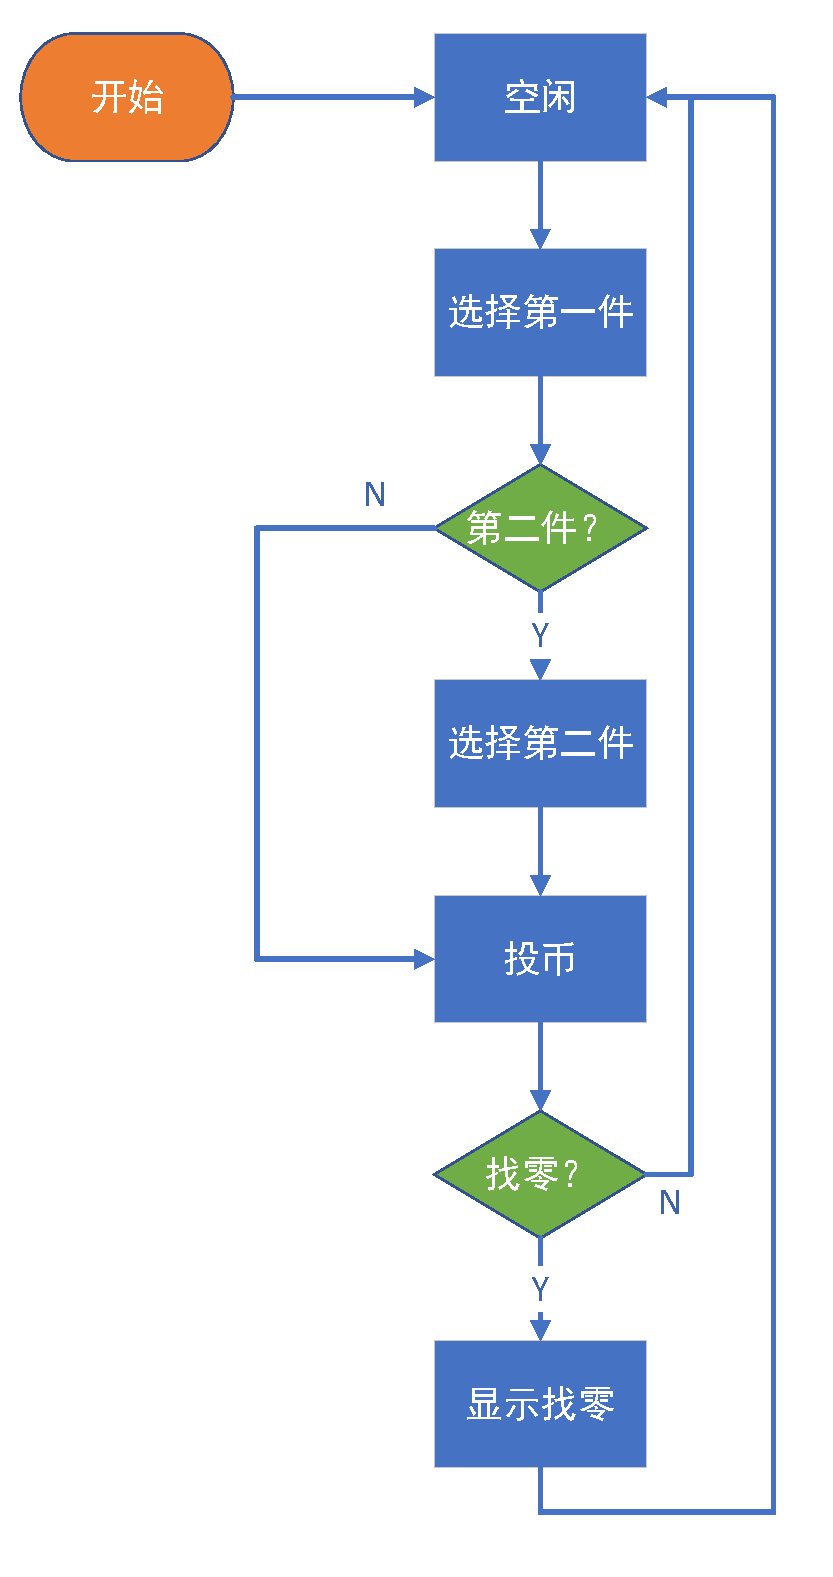
\includegraphics[width=0.5\textwidth]{fig/flowchart.pdf}
        \caption{自动售货机系统架构}
        \label{fig:flowchart}
    \end{figure}
    \section{系统设计}
    \subsection{代码文件列表}
    \begin{itemize}
        \item \texttt{state\_transition.v}:状态机及状态机之间的转换模块;
        \item \texttt{display\_design.v}:显示模块;
        \item \texttt{top\_layer.v}:顶层模块;
        \item \texttt{key\_filter.v}:按键消抖部分;
        \item 其他文件:测试文件、测试脚本等。
    \end{itemize}
    \subsection{状态机设计}
    为了实现自动售货机的功能,我们使用了\texttt{两层状态机}进行实现。在 Verilog 设计中,可以通过\texttt{case-when}语句或者\texttt{if-else}语句实现状态机的功能。两层状态机的各层功能如下:
    \begin{enumerate}
        \item \textbf{第一层状态机}:完成六个状态的切换,包括空闲、商品选择、结账、找零、退出、空闲状态。
        \item \textbf{第二层状态机}:分多个\texttt{always}块,分别完成商品选择、结账、找零、退出状态的具体功能(空闲状态的功能由第一层状态机完成)。
    \end{enumerate}

    下面将具体描述该状态机实现的功能和转换条件。

    \subsubsection{状态机功能描述}
    \textbf{空闲状态(IDLE):}

    初始状态。允许用户按下“确认”键进入商品选择状态。投入钱币数被初始化为0。


    \textbf{商品选择状态(GOODS\_one):}

    用户选择第一件商品,输入购买的商品编号和数量,系统将基于此计算总钱数。用户可以继续按下“选择”键选择第二件商品,或按下“确认”键进入结账状态。
    
    空闲状态下,系统处于待机状态,等待用户的操作。在该状态下,用户一旦按下“确认”键,系统将进入商品选择状态。
    
    \textbf{商品选择状态(GOODS\_two):}

    用户选择第二件商品,输入购买的商品编号和数量,系统将基于此计算总钱数。用户可以继续按下“取消“键退回第一件商品选择,或按下“确认”键进入结账状态。

    \textbf{结账状态(PAYMENT):}

    用户确认购买的商品,系统将根据用户的支付金额,结算购物车中的商品。用户通过按键输入钱数,系统将计算总钱数(并显示),按下“确认”键将进入找零,按下取消键则进入“待定”状态,决定继续选择还是找零退出系统。

    \textbf{找零状态(CHANGE):}

    用户支付的金额超过购买的金额,系统将自动给用户找零。规定用户每次找零不超过1元(按CHANGE键),直至找零完毕,系统退回到初始状态(IDLE)。

    \textbf{待定状态(TEMP):}

    该状态用于决定是否继续选择商品,或是进行找零,退出所有在结账时输入的钱数后,系统回到初始状态。按下“找零”键将进入找零状态,按下“确认”键将回到商品1选择。
    \subsubsection{状态机功能验证}
    使用 \texttt{vscode} 中的 \texttt{TerosHDL} 插件内置的状态机分析模块,我们可以很方便地生成 Verilog 代码对应状态机的状态转移图。经过比较,和理论设计的状态转移图进行了对比,发现两者转移图的状态数量、状态转移方向、状态转移条件等都一致。
    \begin{figure}[htbp]
        \centering
        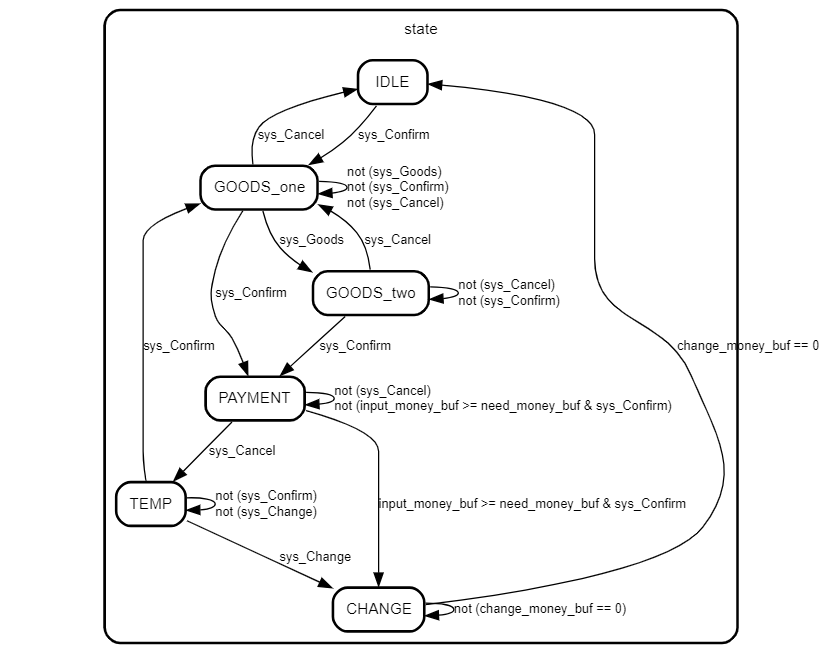
\includegraphics[width=0.75\textwidth]{fig/generatedFlowchart.png}
        \caption{状态转移图}
    \end{figure}

    \subsection{按键消抖设计}
    \subsection{显示模块设计}
    \subsection{I/O接口设计}
    为了便于自动售货机的硬件实现,需要设计可以映射到FPGA主板上的I/O接口。我们使用了如下的接口:
    \begin{itemize}
        \item 五个按键:分别为“确认”、“取消”、“复位”、“找零”、“商品选择”;
        \item 五个拨片输入:分别为“1元”、“5元”、“10元”、“20元”、“50元”;
        \item 八个拨片输入:对应商品编号的六位二进制数,以及购买数量。
    \end{itemize}
    \section{仿真与实物验证}
    \subsection{仿真}
    我们使用Vivado的仿真功能对自动售货机进行了仿真,并通过测试验证了其功能。

    值得一提的是,在仿真时,我们尝试使用 Vscode 中的 TerosHDL 插件进行仿真。TerosHDL 支持对项目进行仿真,并可以生成波形图。但由于其需要安装的附加组件较多,我们最终放弃了这个想法。
    \subsection{实物验证}
    将程序烧录至FPGA主板上,并连接上电源,测试其功能。
    \section{总结}
    \newpage
    \appendix

    \section{项目发布}
    该项目的工程文件及本报告已经上传到Github上,项目地址为:\url{https://github.com/LiPtP0000/Micro-Vending-Machine},包含了本项目的所有代码以及仿真测试文件。
    \section{项目代码列表}
    
\end{document}
